\begin{problem}{Konunglegur Matur}{Inn}{Út}{~}{~}

	\begin{wrapfigure}{r}{0.25\textwidth}
		\vspace{-25pt}
		\begin{center}
			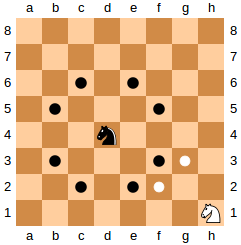
\includegraphics[scale=0.5]{../KonunglegurMatur/skak_riddari.png}
		\end{center}
		\vspace{-20pt}
	\end{wrapfigure}

	Hvíti kóngurinn og hvíta drottningin í skáklandi voru að fara að undirbúa kvöldmáltíðina þegar þau taka eftir því að það vantar sósu til að hafa með matnum. Venjulega myndu þau láta riddara skreppa út í búð fyrir sig, en báðir hvítu riddararnir eru í bardaga við svörtu riddarana, og því ekki heima. Kóngurinn og drottningin ákveða því að annaðhvort þeirra fer út í búð á meðan sá sem bíður heima leggur á borðið. En þau eru bæði orðin mjög svöng, þannig þau vilja að sá sem er fljótari að fara út í búð fari.

	Skákland er í rauninni bara skákborð af stærð $N\times N$. Konungsfjölskyldan er staðsett á reitnum $(s_r, s_c)$, á meðan búðin er staðsett á reitnum $(t_r, t_c)$. Þegar kóngurinn og drottningin eru að ferðast, þá taka þau skref. Í einu skrefi getur kóngurinn farið einn áfram í hvaða átt sem er (og þá eru áttirnar á ská líka teknar með), á meðan að drottningin getur í einu skrefið farið eins marga áfram og hún vill í hvaða átt sem er (og þá eru áttirnar á ská líka teknar með). Athuga skal að þessi skref eru alveg eins í hefðbundinni skák fyrir kóng og drottningu. Líka skal athuga að hvorki kóngurinn né drottningin mega fara úr skáklandi þegar þau eru að taka skref.

	Skrifið forrit sem les inn $N$, $t_r$, $t_c$, $s_r$ og $s_c$, og skrifar út hver þarf færri skref til að komast út í búð, og lætur vita ef skrefafjöldi er sá sami fyrir bæði kónginn og drottninguna.

	\Input
		Á fyrstu línu er heiltalan $1 \leq T \leq 100$, sem táknar fjölda prófunartilvika sem fylgja. Hvert prófunartilvik samanstendur af einni línu með heiltölunum $1 \leq N \leq 1000000, 1 \leq t_r, t_c, s_r, s_c \leq N$.

	\Output

		Fyrir hvert prófunartilvik á að skrifa út eina línu sem inniheldur "`\texttt{King}"' ef kóngurinn þarf færri skref til að komast út í búð, "`\texttt{Queen}"' ef drottningin þarf færri skref til að komast út í búð, en "`\texttt{Same}"' ef drottningin og kóngurinn þurfa jafn mörg skref til að komast út í búð.

	\Examples

		\begin{example}
			\exmp{
2
8 4 4 2 2
100 50 50 50 50
			}{
Queen
Same
}%
		\end{example}

	\Explanation

		Í fyrra prófunartilvikinu eru kóngurinn og drottningin staðsett á reitnum $(4, 4)$, en búðin er staðsett á reitnum $(2,2)$. Þá getur drottningin farið í búðina í einu skrefi, á meðan kóngurinn þarf tvö skref til að fara í búðina.

		Í seinna prófunartilvikinu eru kóngurinn og drottningin staðsett á reitnum $(50, 50)$, en það er sami reitur og búðin er á. Bæði drottningin og kóngurinn þurfa því bæði engin skref til að fara í búðina.

\end{problem}
